% Auto-generated by experiments/make_paper_assets.py
% Requires: booktabs, multirow, graphicx (resizebox).
% Figures first, then the three tables.
% There is no figure 7 onward. The template's 07 pareto, 08 p_harmful
% strip, 09 loss_reduction and 10 combined have no counterpart here:
% 07 and 10 rest on framing the significance tests do not support, 08
% needs mean p_harmful which was dropped, and 09 needs the filler-suffix
% control that only ever ran for the 1B.

% ============================================================
% FIGURE 1: ASR Bar Chart
% ============================================================

\begin{figure}[t]
\centering
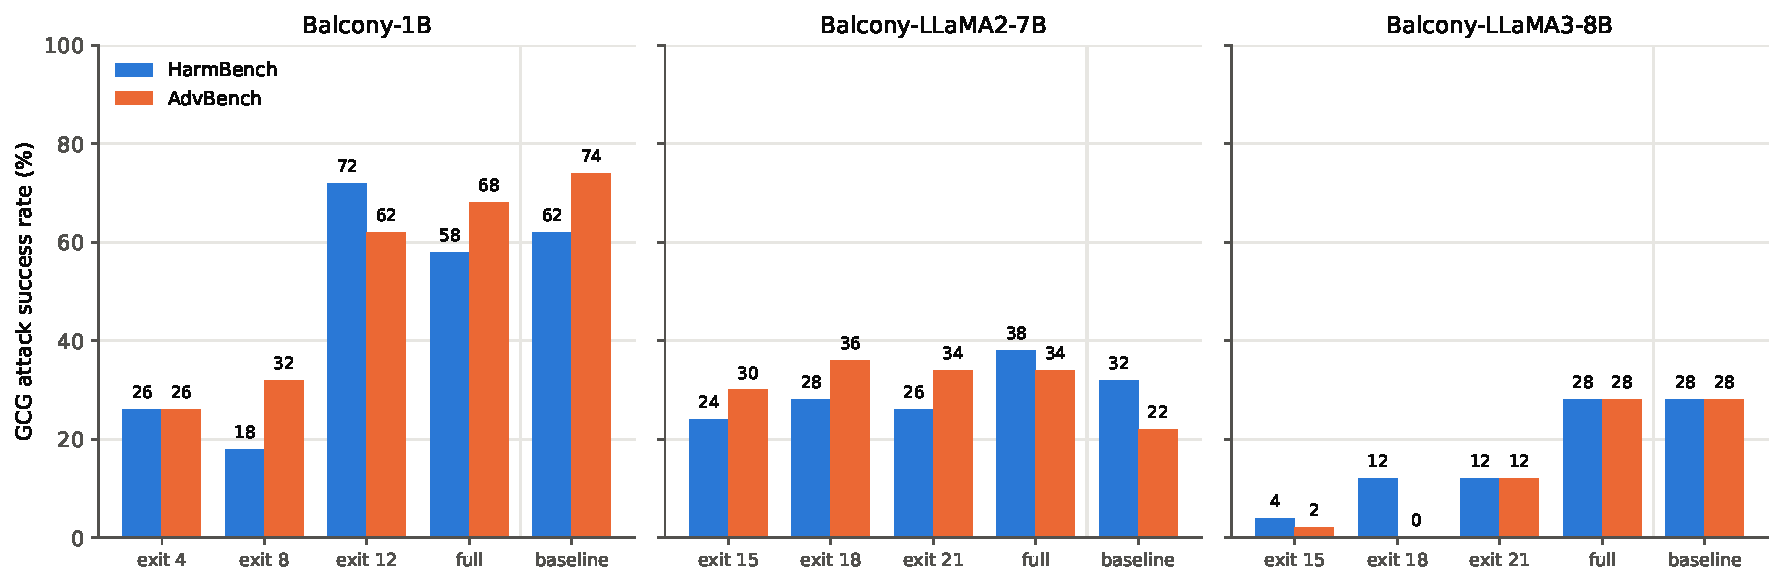
\includegraphics[width=0.85\columnwidth]{paper_figures/01_asr_bar.pdf}
\caption{Attack success rate for every exit of the three models on HarmBench and AdvBench, using GCG with 150 steps on 50 behaviors. ASR is the share of behaviors the HarmBench judge scores above 0.5. The rightmost pair in each panel is that model's no-balcony baseline.}
\label{fig:asr_bar}
\end{figure}

% ============================================================
% FIGURE 2: GCG Loss Curves (HarmBench)
% ============================================================

\begin{figure}[t]
\centering
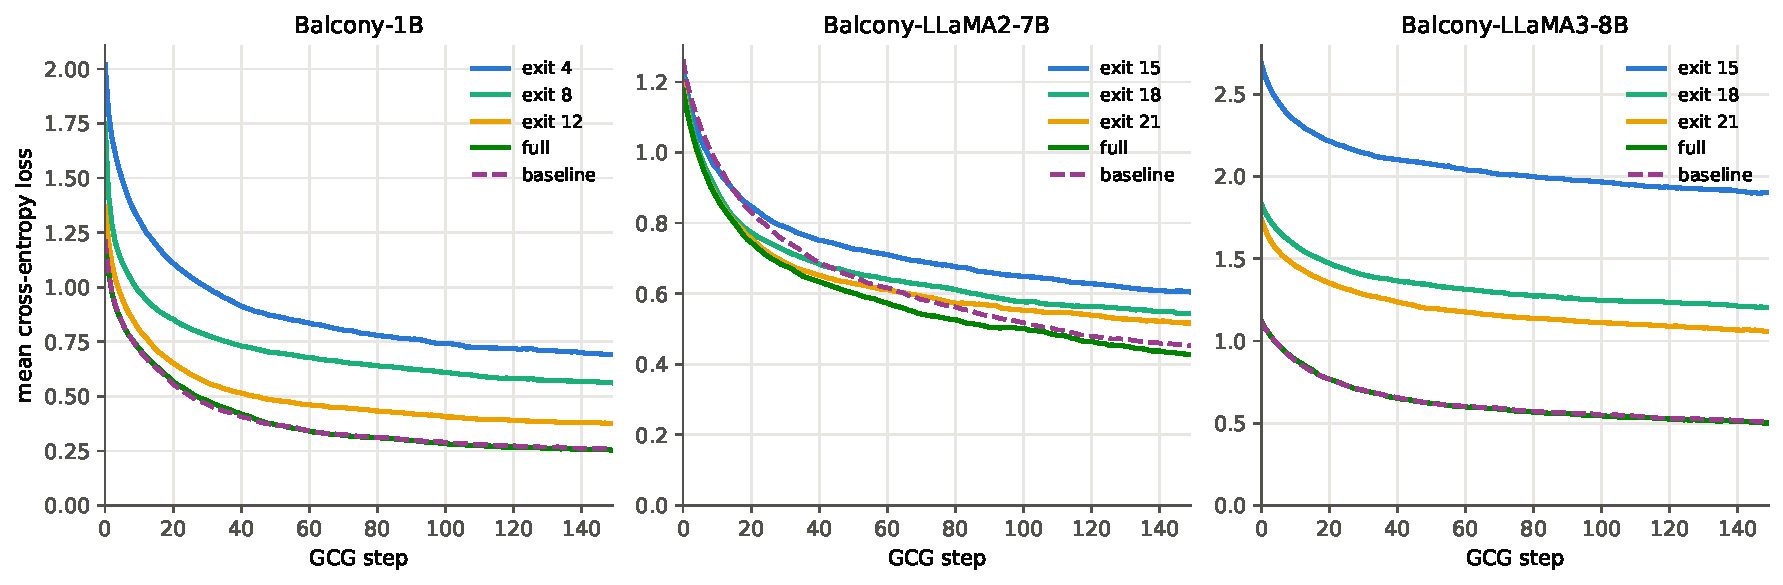
\includegraphics[width=0.85\columnwidth]{paper_figures/02_loss_curves_harmbench.pdf}
\caption{Mean GCG loss across 150 optimization steps on HarmBench, averaged over 50 behaviors, with one line per exit and a separate line for the no-balcony baseline. Most of the drop lands in the first 30 steps and the curves are close to flat by the end.}
\label{fig:loss_curves}
\end{figure}

% ============================================================
% FIGURE 3: GCG Loss Curves (AdvBench)
% ============================================================

\begin{figure}[t]
\centering
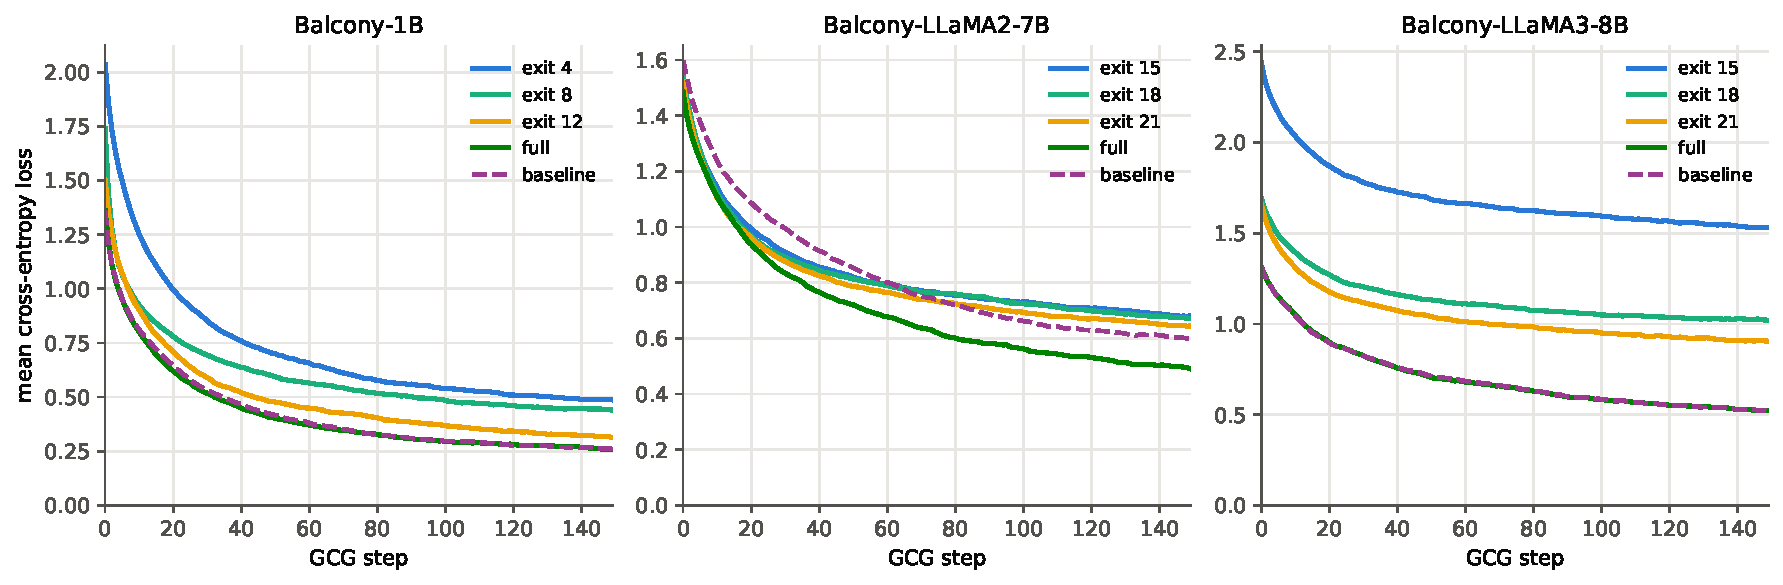
\includegraphics[width=0.85\columnwidth]{paper_figures/03_loss_curves_advbench.pdf}
\caption{The same GCG loss curves on AdvBench. The exits keep the same ordering as on HarmBench, with deeper exits reaching lower final loss.}
\label{fig:advbench_loss_curves}
\end{figure}

% ============================================================
% FIGURE 4: Utility, Clean vs Attacked
% ============================================================

\begin{figure}[t]
\centering
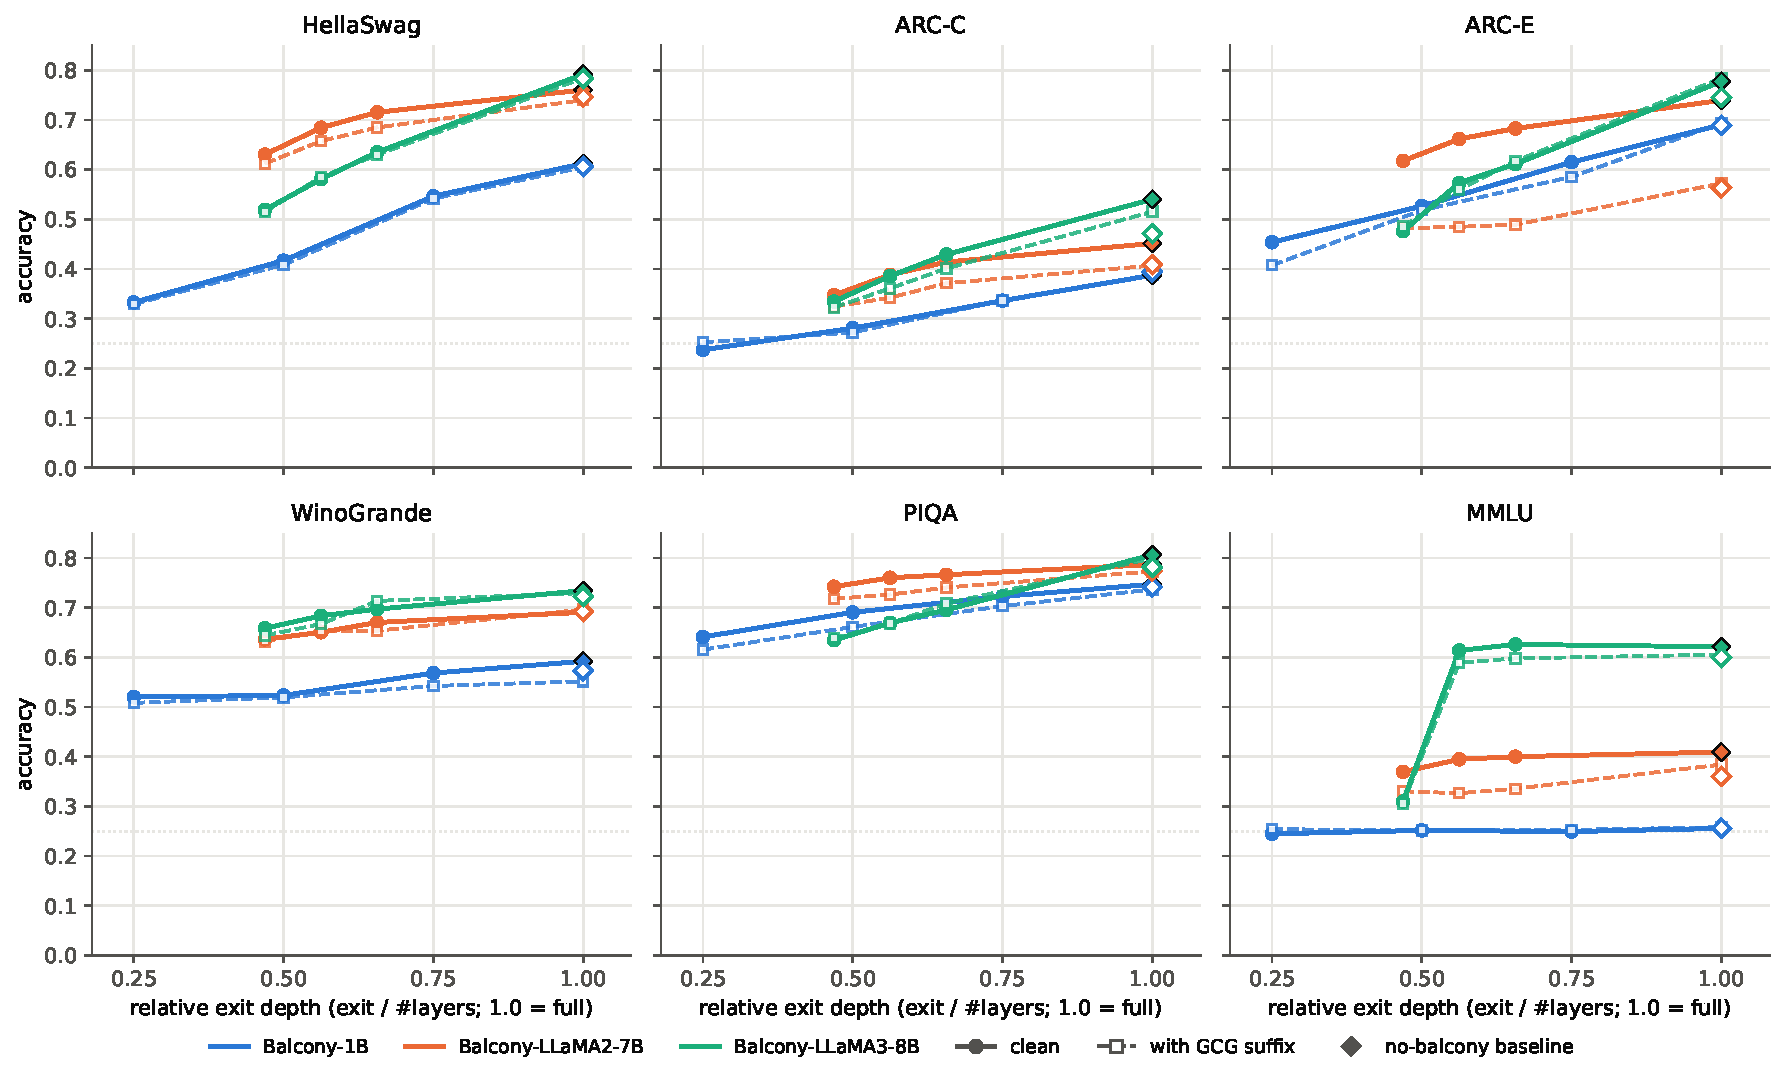
\includegraphics[width=\columnwidth]{paper_figures/04_utility_clean_vs_attacked.pdf}
\caption{Utility on the six benchmarks against relative exit depth, clean (solid) and with the strongest GCG suffix attached (dashed). Each color is one model. The no-balcony baseline is drawn as a diamond at depth 1.0, and on the clean runs it lands on the full model because the two share weights.}
\label{fig:utility_comparison}
\end{figure}

% ============================================================
% FIGURE 5: Final Loss vs ASR
% ============================================================

\begin{figure}[t]
\centering
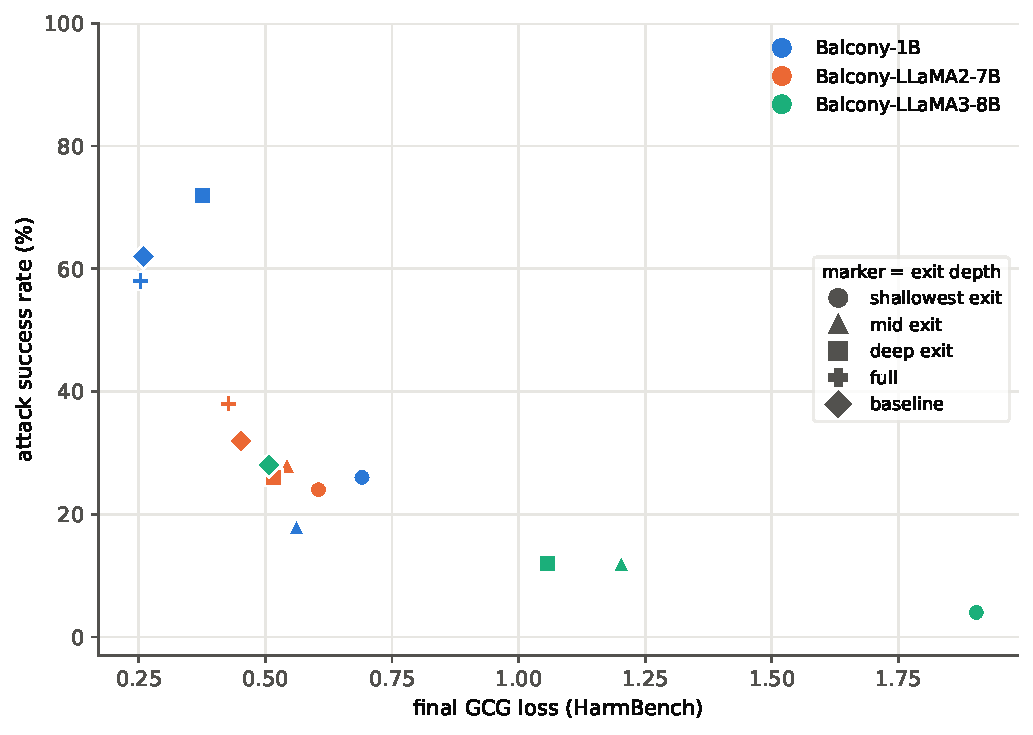
\includegraphics[width=0.75\columnwidth]{paper_figures/05_loss_vs_asr.pdf}
\caption{Final GCG loss against attack success rate on HarmBench, one point per exit and per baseline. Marker shape gives the exit depth and color gives the model. The arms with the lowest final loss are not the arms with the highest ASR.}
\label{fig:loss_vs_asr}
\end{figure}

% ============================================================
% FIGURE 6: HarmBench vs AdvBench Loss
% ============================================================

\begin{figure}[t]
\centering
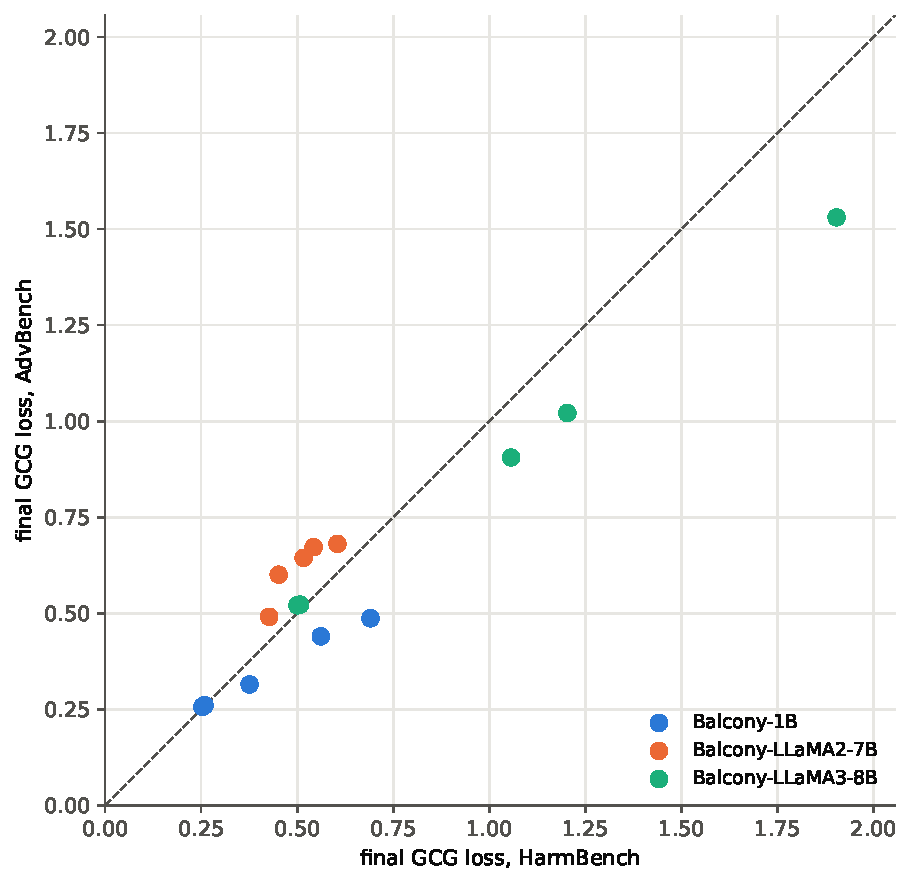
\includegraphics[width=0.7\columnwidth]{paper_figures/06_harmbench_vs_advbench.pdf}
\caption{Final GCG loss on HarmBench against AdvBench for each exit and baseline. The dashed line is y equals x. Points below it reached a lower loss on AdvBench.}
\label{fig:harmbench_vs_advbench}
\end{figure}

% ============================================================
% TABLE 1: Utility Benchmarks, No Attack
% ============================================================

\begin{table}[t]
\centering
\caption{Utility on six multiple choice benchmarks with no attack, for every exit of each model together with the full model and the separate no-balcony baseline. Scores are accuracy from lm-eval-harness (acc\_norm for HellaSwag, ARC and PIQA, acc for WinoGrande and MMLU). The full exit and the no-balcony baseline share trunk weights, so their scores match.}
\label{tab:utility_clean}
\small
\resizebox{\columnwidth}{!}{
\begin{tabular}{ll cccccc}
\toprule
\textbf{Model} & \textbf{Exit} & HellaSwag & ARC-C & ARC-E & WinoGrande & PIQA & MMLU \\
\midrule
\multirow{5}{*}{1B} & Exit 4 & 0.333 & 0.237 & 0.454 & 0.520 & 0.641 & 0.245 \\
 & Exit 8 & 0.417 & 0.281 & 0.527 & 0.523 & 0.690 & 0.252 \\
 & Exit 12 & 0.546 & 0.336 & 0.615 & 0.568 & 0.723 & 0.249 \\
 & Full (16) & 0.612 & 0.387 & 0.690 & 0.592 & 0.747 & 0.256 \\
 & No-Balcony & 0.612 & 0.387 & 0.690 & 0.592 & 0.747 & 0.256 \\
\midrule
\multirow{5}{*}{7B} & Exit 15 & 0.630 & 0.347 & 0.617 & 0.636 & 0.742 & 0.369 \\
 & Exit 18 & 0.684 & 0.388 & 0.662 & 0.650 & 0.760 & 0.395 \\
 & Exit 21 & 0.715 & 0.414 & 0.683 & 0.670 & 0.766 & 0.400 \\
 & Full (32) & 0.760 & 0.451 & 0.739 & 0.691 & 0.787 & 0.409 \\
 & No-Balcony & 0.760 & 0.451 & 0.739 & 0.691 & 0.787 & 0.409 \\
\midrule
\multirow{5}{*}{8B} & Exit 15 & 0.519 & 0.334 & 0.476 & 0.658 & 0.634 & 0.310 \\
 & Exit 18 & 0.581 & 0.386 & 0.573 & 0.684 & 0.669 & 0.614 \\
 & Exit 21 & 0.635 & 0.429 & 0.611 & 0.697 & 0.695 & 0.626 \\
 & Full (32) & 0.792 & 0.540 & 0.777 & 0.734 & 0.806 & 0.621 \\
 & No-Balcony & 0.792 & 0.540 & 0.777 & 0.734 & 0.806 & 0.621 \\
\bottomrule
\end{tabular}}
\end{table}

% ============================================================
% TABLE 2: Utility Under Attack
% ============================================================

\begin{table}[t]
\centering
\caption{Utility with each exit's strongest GCG suffix appended to every question. Numbers in parentheses are the change from the clean scores in Table~\ref{tab:utility_clean}, in percentage points. Most cells move by under 3 points. The exception is ARC-E on the 7B, which drops between 13 and 19 points at every arm, including the full model and the no-balcony baseline.}
\label{tab:utility_attacked}
\small
\resizebox{\columnwidth}{!}{
\begin{tabular}{ll cccccc}
\toprule
\textbf{Model} & \textbf{Exit} & HellaSwag & ARC-C & ARC-E & WinoGrande & PIQA & MMLU \\
\midrule
\multirow{5}{*}{1B} & Exit 4 & 0.329 \scriptsize{($-$0.3)} & 0.253 \scriptsize{(+1.5)} & 0.407 \scriptsize{($-$4.6)} & 0.508 \scriptsize{($-$1.2)} & 0.615 \scriptsize{($-$2.6)} & 0.254 \scriptsize{(+0.9)} \\
 & Exit 8 & 0.409 \scriptsize{($-$0.8)} & 0.272 \scriptsize{($-$0.9)} & 0.518 \scriptsize{($-$0.8)} & 0.519 \scriptsize{($-$0.4)} & 0.661 \scriptsize{($-$2.9)} & 0.252 \scriptsize{(+0.0)} \\
 & Exit 12 & 0.542 \scriptsize{($-$0.5)} & 0.336 \scriptsize{(+0.0)} & 0.585 \scriptsize{($-$2.9)} & 0.542 \scriptsize{($-$2.6)} & 0.703 \scriptsize{($-$2.0)} & 0.253 \scriptsize{(+0.3)} \\
 & Full (16) & 0.605 \scriptsize{($-$0.7)} & 0.388 \scriptsize{(+0.1)} & 0.694 \scriptsize{(+0.3)} & 0.552 \scriptsize{($-$4.0)} & 0.737 \scriptsize{($-$1.0)} & 0.258 \scriptsize{(+0.2)} \\
 & No-Balcony & 0.606 \scriptsize{($-$0.6)} & 0.394 \scriptsize{(+0.7)} & 0.689 \scriptsize{($-$0.1)} & 0.573 \scriptsize{($-$1.9)} & 0.742 \scriptsize{($-$0.5)} & 0.256 \scriptsize{(+0.0)} \\
\midrule
\multirow{5}{*}{7B} & Exit 15 & 0.612 \scriptsize{($-$1.8)} & 0.324 \scriptsize{($-$2.3)} & 0.482 \scriptsize{($-$13.6)} & 0.632 \scriptsize{($-$0.4)} & 0.718 \scriptsize{($-$2.4)} & 0.330 \scriptsize{($-$3.9)} \\
 & Exit 18 & 0.657 \scriptsize{($-$2.7)} & 0.342 \scriptsize{($-$4.6)} & 0.485 \scriptsize{($-$17.7)} & 0.653 \scriptsize{(+0.2)} & 0.726 \scriptsize{($-$3.4)} & 0.326 \scriptsize{($-$6.8)} \\
 & Exit 21 & 0.685 \scriptsize{($-$3.0)} & 0.371 \scriptsize{($-$4.3)} & 0.489 \scriptsize{($-$19.4)} & 0.654 \scriptsize{($-$1.7)} & 0.740 \scriptsize{($-$2.6)} & 0.335 \scriptsize{($-$6.5)} \\
 & Full (32) & 0.740 \scriptsize{($-$2.0)} & 0.407 \scriptsize{($-$4.4)} & 0.572 \scriptsize{($-$16.7)} & 0.696 \scriptsize{(+0.6)} & 0.773 \scriptsize{($-$1.4)} & 0.384 \scriptsize{($-$2.5)} \\
 & No-Balcony & 0.746 \scriptsize{($-$1.4)} & 0.409 \scriptsize{($-$4.3)} & 0.563 \scriptsize{($-$17.6)} & 0.692 \scriptsize{(+0.2)} & 0.774 \scriptsize{($-$1.3)} & 0.360 \scriptsize{($-$4.9)} \\
\midrule
\multirow{5}{*}{8B} & Exit 15 & 0.515 \scriptsize{($-$0.4)} & 0.323 \scriptsize{($-$1.2)} & 0.485 \scriptsize{(+0.9)} & 0.644 \scriptsize{($-$1.4)} & 0.638 \scriptsize{(+0.4)} & 0.306 \scriptsize{($-$0.4)} \\
 & Exit 18 & 0.585 \scriptsize{(+0.4)} & 0.361 \scriptsize{($-$2.5)} & 0.560 \scriptsize{($-$1.3)} & 0.667 \scriptsize{($-$1.7)} & 0.668 \scriptsize{($-$0.1)} & 0.589 \scriptsize{($-$2.5)} \\
 & Exit 21 & 0.629 \scriptsize{($-$0.5)} & 0.401 \scriptsize{($-$2.8)} & 0.617 \scriptsize{(+0.6)} & 0.713 \scriptsize{(+1.7)} & 0.708 \scriptsize{(+1.3)} & 0.598 \scriptsize{($-$2.8)} \\
 & Full (32) & 0.785 \scriptsize{($-$0.7)} & 0.515 \scriptsize{($-$2.5)} & 0.784 \scriptsize{(+0.7)} & 0.729 \scriptsize{($-$0.5)} & 0.799 \scriptsize{($-$0.7)} & 0.605 \scriptsize{($-$1.6)} \\
 & No-Balcony & 0.783 \scriptsize{($-$0.8)} & 0.471 \scriptsize{($-$6.9)} & 0.745 \scriptsize{($-$3.2)} & 0.722 \scriptsize{($-$1.2)} & 0.781 \scriptsize{($-$2.5)} & 0.600 \scriptsize{($-$2.1)} \\
\bottomrule
\end{tabular}}
\end{table}

% ============================================================
% TABLE 3: Main Attack Results
% ============================================================

\begin{table}[t]
\centering
\caption{GCG attack results on both benchmarks. Final loss is the mean cross entropy GCG minimizes over 50 behaviors after 150 steps. ASR is the share of those behaviors the HarmBench judge scores above 0.5. Each model is listed for every exit, the full model, and its no-balcony baseline.}
\label{tab:attack_results}
\small
\resizebox{\columnwidth}{!}{
\begin{tabular}{ll cccc}
\toprule
\textbf{Model} & \textbf{Exit} & HB Loss & HB ASR\% & AB Loss & AB ASR\% \\
\midrule
\multirow{5}{*}{1B} & Exit 4 & 0.691 & 26.0 & 0.487 & 26.0 \\
 & Exit 8 & 0.562 & 18.0 & 0.440 & 32.0 \\
 & Exit 12 & 0.376 & 72.0 & 0.315 & 62.0 \\
 & Full (16) & 0.253 & 58.0 & 0.257 & 68.0 \\
 & No-Balcony & 0.259 & 62.0 & 0.261 & 74.0 \\
\midrule
\multirow{5}{*}{7B} & Exit 15 & 0.605 & 24.0 & 0.681 & 30.0 \\
 & Exit 18 & 0.543 & 28.0 & 0.672 & 36.0 \\
 & Exit 21 & 0.517 & 26.0 & 0.644 & 34.0 \\
 & Full (32) & 0.427 & 38.0 & 0.491 & 34.0 \\
 & No-Balcony & 0.452 & 32.0 & 0.600 & 22.0 \\
\midrule
\multirow{5}{*}{8B} & Exit 15 & 1.904 & 4.0 & 1.530 & 2.0 \\
 & Exit 18 & 1.203 & 12.0 & 1.021 & 0.0 \\
 & Exit 21 & 1.057 & 12.0 & 0.906 & 12.0 \\
 & Full (32) & 0.501 & 28.0 & 0.521 & 28.0 \\
 & No-Balcony & 0.507 & 28.0 & 0.522 & 28.0 \\
\bottomrule
\end{tabular}}
\end{table}
